%!TEX program = lualatex
\documentclass[14pt]{constructor-diploma}

\usepackage[backend=bibtex]{biblatex}
\usepackage{minted}
\usepackage{mdframed}
\usepackage{physics}
\usepackage{amsmath}
\usepackage{tikz}
\usepackage{mathdots}
\usepackage{yhmath}
\usepackage{cancel}
\usepackage{color}
\usepackage{siunitx}
\usepackage{array}
\usepackage{multirow}
\usepackage{amssymb}
\usepackage{gensymb}
\usepackage{tabularx}
\usepackage{extarrows}
\usepackage{booktabs}
\usetikzlibrary{fadings}
\usetikzlibrary{patterns}
\usetikzlibrary{shadows.blur}
\usetikzlibrary{shapes}


\usemintedstyle{tango}

\addbibresource{diploma.bib}

\begin{document}
% Год, город, название университета и факультета предопределены,
% но можно и поменять.
% Если англоязычная титульная страница не нужна, то ее можно просто удалить.
\filltitle{en}{
    chair              = {Bachelor of Science \\ Computer Science},
    title              = {Mechanized verification of pretty-printing library implemented in C},
    author             = {Ivan Klimov},
    supervisorPosition = {Prof.},
    supervisor         = {Anton Podkopaev},
    reviewerPosition   = {},
    reviewer           = {},
}
\maketitle
\tableofcontents
% У введения нет номера главы
\section*{Introduction}
Pretty-printing is a technique used to format code or data in a human-readable way.
It involves adding indentation, line breaks, and other formatting elements to make code or data more visually organized and easier to understand.
Particulary, we will be interested in pretty-printers, 
which transform code from some abstract representation of a program(for example, AST)
into comprehensible text that satisfies certain properties.

When code is formatted in a way that is easy to read,
developers can quickly identify errors or inconsistencies, 
making debugging and troubleshooting faster and more efficient.
Additionally, well-formatted code is easier to modify, update, and maintain over time, 
as changes can be made with confidence that they will not accidentally affect other parts of the codebase.

Since pretty-printing become an essential tool for any developer looking to create code, many algorithms, that are using different techniques and different asymptotics to achieve the desired result,
have emerged~\cite{oppen,azero,hughes,swierstra,podkopaev,bernardy}. Particulary in the area of functional programming, algorithms based on pretty-printing combinators have appeared,
allowing very natural way of working with text representation of AST. 
Wadler~\cite{wadler} and Hughes'~\cite{hughes} libraries stand out among them, as they are included in the standard libraries of Ocaml and Haskell.
However, these algorithms are not the most powerful in terms of expressive power, and are less efficient than existing counterparts.

A more flexible approach is \textit{pretty-printer combinators with choice},
providing more freedom when working with combinators and thus allowing to put more constraints on the solutions obtained
as a result of the algorithm.
Pretty-printer combinators with choice (we will be calling them printers in further reading) were originally presented in the works of Pablo Azero and Doaitse Swierstra~\cite{azero, swierstra}, 
however, their proposed algorithm has exponential complexity in the worst case. Significant impovements have been made in 
libraries of Anton Podkopaev and Dmitri Boulytchev~\cite{podkopaev} and Jean-Philippe Bernardy~\cite{bernardy}, algorithms in which are polynomial.

Bugs in algorithm implementations can lead to many problems, such as loss of information during formatting,
mismatch between the resulting text and the given parameters, etc. Therefore, it is important to verify 
the code that is used to format data.
Among recent results: a Vladimir Korolikhins' verified library of printers~\cite{korolihin} in Coq, an interactive proof assistant, 
providing a formal language to write mathematical definitions, executable algorithms and theorems together with an environment for semi-interactive development of machine-checked proofs. 
The library includes different functional pretty-printing algorithms,
starting from the simple but less efficient algorithm by Pablo Azero and ending 
with more advanced polynomial algorithms by Anton Podkopaev and Dmitri Boulytchev~\cite{podkopaev} and Jean-Philippe Bernardy~\cite{bernardy}.

However, all verified versions of pretty-printing libraries are functional. 
% Implementing a verified pretty-printer library in C and further expanding it with a polynomial algorithm 
% will allow us to achieve significant performance improvements. This will be the main goal of our work.
Implementing a verified pretty-printer library in C will allow us to optimize the written code more efficiently, and in the future 
expand the library with a polynomial algorithm, which will result in hopefully more perfomant implementation than its existing functional counterparts.
This will be the main goal of our work.

\section{Goals and objectives}
The goal of this work is to provide a verified implementation of pretty-printer combinators library in C. 
The algorithm that we are going to implement and verify 
is described in article of Swierstra et al.~\cite{swierstra}. 
It has exponential complexity in the worst case, nevertheless, 
it was chosen because it supports the extension of functionality, 
as the algorithm is based on the same approach (pretty-printer combinators with choice) 
as more advanced polynomial algorithms~\cite{podkopaev,bernardy}. 

After implementing the library in C, we will need to verify it. 
To do this, we will prove the correspondence between our library and Korolikhin's verified library~\cite{korolihin} in Coq (which was chosen due to the absence of analogs, as well as the presence in this library of the algorithm we are going to implement).
We will divide this part into two subtasks. 

Firstly, we will need to verify the basic structures for working with printer combinators, as well as the printer combinators themselves. 
This will allow us to already at that point be able to extend the library with any algorithm based on pretty-printer combinators.

Secondly, we will need to verify the algorithm itself, in which at that point the printer combinators will already be verified and 
it will only remain to prove statements about the highest-level functions that manipulate printer combinators.
Thus, the main objectives of this work are:

\begin{enumerate}
  \item Implement the pretty-printer library~\cite{swierstra} in C.
  \item Prove that the C implementation of the core operations on Formats and combinators satisfy its functional specification~\cite{korolihin}.
  \item Extend the proof to verify the correctness of the chosen algorithm~\cite{swierstra}.
\end{enumerate}


\section{Related work}

\subsection{Pretty-printing library}

This sections aims to give detailed explanation of pretty-printing library, described in article by Swierstra et al.~\cites{swierstra} 
and all the approaches that are used in it, including detailed description of pretty-printer combinators.

% \label{section_brief}
% \subsubsection{Brief overview}
% The algorithm takes as input a representation of the text in the form of an AST, and for each node, 
% it constructs a list of possible formatted text pieces. 
% Each formatted text piece is stored in a structure called \textit{format}. 
% In addition to the text itself, the format contains some properties of the formatted data for ease of further manipulation with the structure.
% The combination of formats is done using \textit{pretty-printing combinators}, 
% which are essentially functions that take two formats as arguments
% and return a new format that represents formatted concatenation of the two original text pieces. 
% The algorithm uses printer combinators to iterate through all possible formatting options for the data. 
% In other words, the node of the AST is associated with not a single format, 
% but a list of formats that are all possible ways to format the data corresponding to that node. 
% In each of the AST leaves, there is list of a single element (the format, which is essentially a string), 
% and during recursive runs, all possible formats of the left and right children are iterated through, 
% and all possible combinations of combinators are applied to them. 
% At the end of the algorithm, we choose the most suitable format for us from the root node.

\subsubsection{Description of the \texttt{Format} structure}
The atomic structure when working with printer combinators is the \texttt{Format} structure. 
\begin{figure}[H]
\definecolor{bg}{rgb}{0.95,0.95,0.95}

\begin{mdframed}[backgroundcolor=bg]
\begin{minted}[fontsize=\small]{coq}
Record format : Type := Format {
  height           : nat;
  first_line_width : nat;
  middle_width     : nat;
  last_line_width  : nat;
  to_text          : nat -> string -> string
}.
\end{minted}
\end{mdframed}
\caption{\texttt{Format} definition in the reference library~\cite{korolihin}}
\label{fig:format}
\end{figure}
This structure represents pre-formatted text that includes the following parameters:

\begin{enumerate}
  \item \textbf{Height} of the Format. This parameter is used to determine the number of lines in the formatted text.
  \item \textbf{First line width} of the Format. This parameter is used to determine the width of the first line of the formatted text.
  \item \textbf{Middle line width} of the Format. This parameter is used to determine the maximum width of all the lines between first and last lines.
  If there's only two lines in the formatted text, then this parameter is equal to the first line width. 
  If there's only one line in the formatted text, then this parameter is equal to the width of this line.
  \item \textbf{Last line width} of the Format. This parameter is used to determine the width of the last line of the formatted text.
  \item \textbf{\texttt{to\_text}} function allows obtaining text representation of the Format. 
  The \texttt{to\_text} function takes two arguments: 
  \texttt{shift}, which specifies the desired shift of the text representation, and \texttt{line}, 
  which will be appended to our text representation.
  In particular, by taking a shift equal to zero and an empty string as a line, we obtain an exact textual representation of the formatted data.
\end{enumerate}

As an illustration, we'll give an example of a specific Format and the information it contains. 
Suppose we want to format the following piece of \texttt{C++} code:

\begin{figure}[H]
\definecolor{bg}{rgb}{0.95,0.95,0.95}

\begin{mdframed}[backgroundcolor=bg]
\begin{minted}[fontsize=\small]{cpp}
int s;
if(condition1) { s = 1; } else if(condition2) { s = 2; }
\end{minted}
\end{mdframed}
\caption{Sample of \texttt{C++} code}
\end{figure}

This code can be formatted in many different ways. 
Let's consider the Format \texttt{G} and say that it contains the following representation of our code:

\begin{figure}[H]
\definecolor{bg}{rgb}{0.95,0.95,0.95}

\begin{mdframed}[backgroundcolor=bg]
\begin{minted}[fontsize=\small,linenos]{cpp}
int s;
if(condition1) { 
  s = 1; 
} else if(condition2) { 
  s = 2; 
}
\end{minted}
\end{mdframed}
\caption{Formatted \texttt{C++} code}
\label{fig:format_text}
\end{figure}

We will go through all the Format's fields and calculate values for them:

\begin{enumerate}
  \item \texttt{G.height}. As shown in the Figure~\ref{fig:format_text}, the amount of lines in 
  the formatted text is equal to 6. Therefore, the height of our Format is equal to 6.
  \item \texttt{G.first\_line\_width}. As shown in the Figure~\ref{fig:format_text}, 
  the first line of the text is \mintinline{cpp}{int s;}. It's width is equal to 6, so 
  the first line width of our Format is also equal to 6.
  \item \texttt{G.middle\_width}. As shown in the Figure~\ref{fig:format_text}, there are 4
  lines that are between the first one and the last one:
\begin{figure}[H]
\begin{minted}[fontsize=\small,linenos]{cpp}
if(condition1) { 
  s = 1; 
} else if(condition2) { 
  s = 2; 
\end{minted}
\end{figure}
\vspace*{-25pt}
  The third one obviously has the maximuum width among them, and it's width equal to 23. So the middle line width 
  of our Format is also equal to 23.
  \item \texttt{G.last\_line\_width}. As shown in the Figure~\ref{fig:format_text}, the last line of the 
  text is \}. It's width is equal to 1, so the last line width of our Format is also equal to 1.
  \item \texttt{G.to\_text}. As we discussed earlier, the \texttt{to\_text} function with default arguments returns the formatted text, shown 
  in Figure~\ref{fig:format_text}. 
  Changing the first parameter affects the indentation of the entire returned text, and changing the second parameter allows modifying the entire text by adding an arbitrary string to the end of it. 
  Later, we will show that these parameters are not necessary for a work with Formats, nevertheless, it is important to understand their semantics as they are used in the reference library.

\begin{figure}[H]
\begin{minipage}{0.5\textwidth}
\definecolor{bg}{rgb}{0.95,0.95,0.95}

\begin{mdframed}[backgroundcolor=bg]
\begin{minted}[fontsize=\small]{cpp}
int s;
if(condition1) { 
  s = 1; 
} else if(condition2) { 
  s = 2; 
}
\end{minted}
\end{mdframed}
% \vspace*{-35pt}
\end{minipage}
\begin{minipage}{0.5\textwidth}
\definecolor{bg}{rgb}{0.95,0.95,0.95}

\begin{mdframed}[backgroundcolor=bg]
\begin{minted}[fontsize=\small]{cpp}
    int s;
    if(condition1) { 
      s = 1; 
    } else if(condition2) { 
      s = 2; 
    } else {
\end{minted}
\end{mdframed}
\end{minipage}
% \vspace*{30pt}
\caption{\texttt{G.to\_text(0, EmptyString)} and \texttt{G.to\_text(5, " else \{")}}
\label{fig:to_text_example}
\end{figure}
\end{enumerate}

Internal representation of our concrete Format is shown in Figure~\ref{fig:format_example}.
We didn't include the specific implementation of \texttt{to\_text} function as it can be implemented 
in many different ways and it's more important to understand its semantics.
\begin{figure}[H]
\definecolor{bg}{rgb}{0.95,0.95,0.95}
\begin{mdframed}[backgroundcolor=bg]
\begin{minted}[fontsize=\small]{coq}
G = 
{|
  height := 6;
  first_line_width := 6;
  middle_width := 23;
  last_line_width := 1;
  to_text := ...
|}
\end{minted}
\end{mdframed}
\caption{Format \texttt{G}}
\label{fig:format_example}
\end{figure}


\label{section_combinators}
\subsubsection{Description of pretty-printer combinators}
\begin{figure}[H]
\begin{center}


\tikzset{every picture/.style={line width=0.75pt}} %set default line width to 0.75pt        

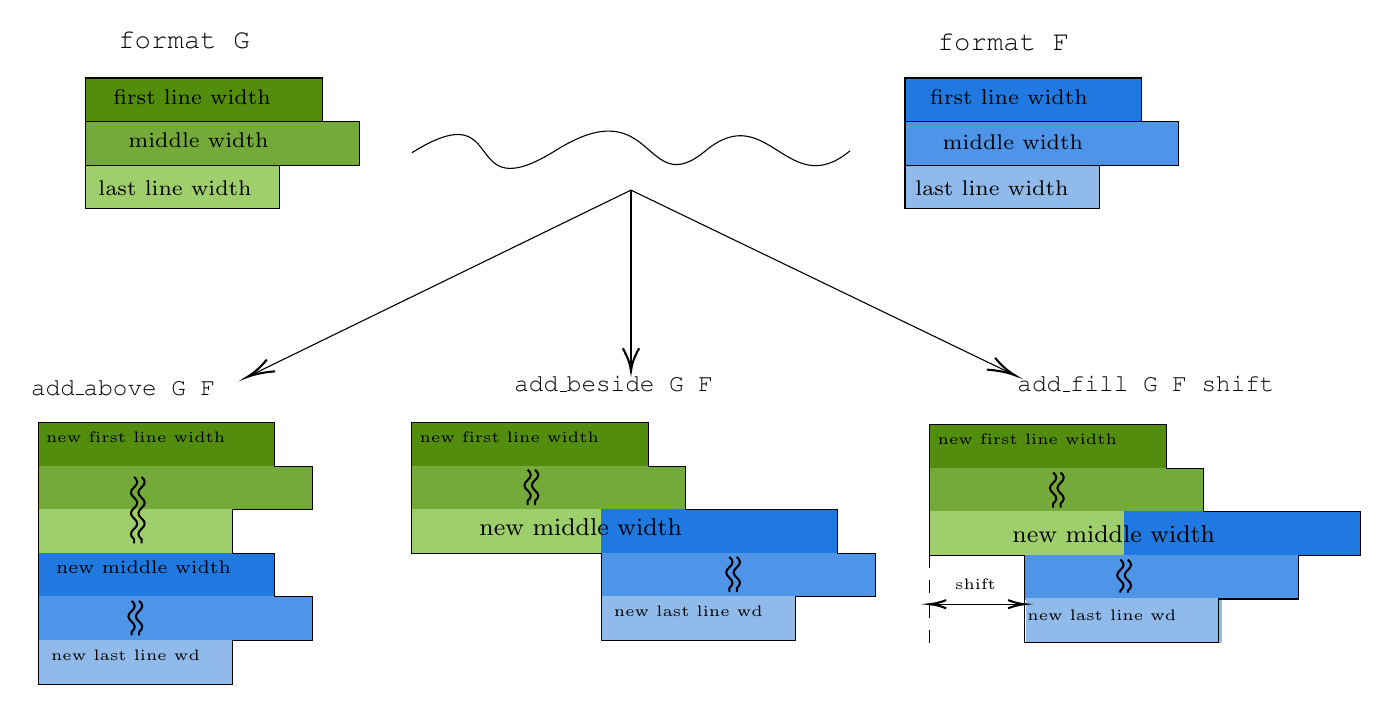
\begin{tikzpicture}[x=0.75pt,y=0.75pt,yscale=-1,xscale=1.2]
%uncomment if require: \path (0,446); %set diagram left start at 0, and has height of 446

%Curve Lines [id:da7282724148856031] 
\draw    (183,102) .. controls (223,72) and (201,130.73) .. (241,100.73) .. controls (281,70.73) and (276,126) .. (301,101) .. controls (326,76) and (334,126) .. (359,101) ;
%Straight Lines [id:da732226138129258] 
\draw    (271,120) -- (423.27,208.11) ;
\draw [shift={(425,209.12)}, rotate = 210.06] [color={rgb, 255:red, 0; green, 0; blue, 0 }  ][line width=0.75]    (10.93,-3.29) .. controls (6.95,-1.4) and (3.31,-0.3) .. (0,0) .. controls (3.31,0.3) and (6.95,1.4) .. (10.93,3.29)   ;
%Straight Lines [id:da2673745236113916] 
\draw    (271,120) -- (271,205.12) ;
\draw [shift={(271,207.12)}, rotate = 270] [color={rgb, 255:red, 0; green, 0; blue, 0 }  ][line width=0.75]    (10.93,-3.29) .. controls (6.95,-1.4) and (3.31,-0.3) .. (0,0) .. controls (3.31,0.3) and (6.95,1.4) .. (10.93,3.29)   ;
%Straight Lines [id:da5590791800548975] 
\draw    (271,120) -- (118.73,208.99) ;
\draw [shift={(117,210)}, rotate = 329.7] [color={rgb, 255:red, 0; green, 0; blue, 0 }  ][line width=0.75]    (10.93,-3.29) .. controls (6.95,-1.4) and (3.31,-0.3) .. (0,0) .. controls (3.31,0.3) and (6.95,1.4) .. (10.93,3.29)   ;
%Shape: Rectangle [id:dp808837789421493] 
\draw  [fill={rgb, 255:red, 82; green, 141; blue, 13 }  ,fill opacity=1 ] (52,66) -- (147,66) -- (147,87) -- (52,87) -- cycle ;
%Shape: Rectangle [id:dp9793592211997744] 
\draw  [fill={rgb, 255:red, 115; green, 170; blue, 57 }  ,fill opacity=1 ] (52,87) -- (162,87) -- (162,108) -- (52,108) -- cycle ;
%Shape: Rectangle [id:dp932877347953496] 
\draw  [fill={rgb, 255:red, 159; green, 207; blue, 109 }  ,fill opacity=1 ] (52,108) -- (130,108) -- (130,129) -- (52,129) -- cycle ;
%Shape: Rectangle [id:dp7757811105837442] 
\draw  [fill={rgb, 255:red, 31; green, 121; blue, 224 }  ,fill opacity=1 ] (381,66) -- (476,66) -- (476,87) -- (381,87) -- cycle ;
%Shape: Rectangle [id:dp9348863965428301] 
\draw  [fill={rgb, 255:red, 78; green, 148; blue, 233 }  ,fill opacity=1 ] (381,87) -- (491,87) -- (491,108) -- (381,108) -- cycle ;
%Shape: Rectangle [id:dp5258984646265605] 
\draw  [fill={rgb, 255:red, 144; green, 186; blue, 234 }  ,fill opacity=1 ] (381,108) -- (459,108) -- (459,129) -- (381,129) -- cycle ;
%Shape: Rectangle [id:dp001902336021333717] 
\draw  [color={rgb, 255:red, 82; green, 141; blue, 13 }  ,draw opacity=1 ][fill={rgb, 255:red, 82; green, 141; blue, 13 }  ,fill opacity=1 ] (33,232) -- (128,232) -- (128,253) -- (33,253) -- cycle ;
%Shape: Rectangle [id:dp4189646464121347] 
\draw  [color={rgb, 255:red, 115; green, 170; blue, 57 }  ,draw opacity=1 ][fill={rgb, 255:red, 115; green, 170; blue, 57 }  ,fill opacity=1 ] (33,253) -- (143,253) -- (143,274) -- (33,274) -- cycle ;
%Shape: Rectangle [id:dp6182085830852484] 
\draw  [color={rgb, 255:red, 159; green, 207; blue, 109 }  ,draw opacity=1 ][fill={rgb, 255:red, 159; green, 207; blue, 109 }  ,fill opacity=1 ] (33,274) -- (111,274) -- (111,295) -- (33,295) -- cycle ;
%Shape: Rectangle [id:dp279035114500889] 
\draw  [color={rgb, 255:red, 31; green, 121; blue, 224 }  ,draw opacity=1 ][fill={rgb, 255:red, 31; green, 121; blue, 224 }  ,fill opacity=1 ] (33,295) -- (128,295) -- (128,316) -- (33,316) -- cycle ;
%Shape: Rectangle [id:dp7094574853653807] 
\draw  [color={rgb, 255:red, 78; green, 148; blue, 233 }  ,draw opacity=1 ][fill={rgb, 255:red, 78; green, 148; blue, 233 }  ,fill opacity=1 ] (33,316) -- (143,316) -- (143,337) -- (33,337) -- cycle ;
%Shape: Rectangle [id:dp6311197532441868] 
\draw  [color={rgb, 255:red, 144; green, 186; blue, 234 }  ,draw opacity=1 ][fill={rgb, 255:red, 144; green, 186; blue, 234 }  ,fill opacity=1 ] (33,337) -- (111,337) -- (111,358) -- (33,358) -- cycle ;
%Shape: Rectangle [id:dp005304650175637082] 
\draw  [color={rgb, 255:red, 82; green, 141; blue, 13 }  ,draw opacity=1 ][fill={rgb, 255:red, 82; green, 141; blue, 13 }  ,fill opacity=1 ] (183,232) -- (278,232) -- (278,253) -- (183,253) -- cycle ;
%Shape: Rectangle [id:dp1795210702408092] 
\draw  [color={rgb, 255:red, 115; green, 170; blue, 57 }  ,draw opacity=1 ][fill={rgb, 255:red, 115; green, 170; blue, 57 }  ,fill opacity=1 ] (183,253) -- (293,253) -- (293,274) -- (183,274) -- cycle ;
%Shape: Rectangle [id:dp281817417555301] 
\draw  [color={rgb, 255:red, 159; green, 207; blue, 109 }  ,draw opacity=1 ][fill={rgb, 255:red, 159; green, 207; blue, 109 }  ,fill opacity=1 ] (183,274) -- (261,274) -- (261,295) -- (183,295) -- cycle ;
%Shape: Rectangle [id:dp2764643146730045] 
\draw  [color={rgb, 255:red, 31; green, 121; blue, 224 }  ,draw opacity=1 ][fill={rgb, 255:red, 31; green, 121; blue, 224 }  ,fill opacity=1 ] (259,274) -- (354,274) -- (354,295) -- (259,295) -- cycle ;
%Shape: Rectangle [id:dp14893535880956488] 
\draw  [color={rgb, 255:red, 78; green, 148; blue, 233 }  ,draw opacity=1 ][fill={rgb, 255:red, 78; green, 148; blue, 233 }  ,fill opacity=1 ] (259,295) -- (369,295) -- (369,316) -- (259,316) -- cycle ;
%Shape: Rectangle [id:dp1374086019688595] 
\draw  [color={rgb, 255:red, 144; green, 186; blue, 234 }  ,draw opacity=1 ][fill={rgb, 255:red, 144; green, 186; blue, 234 }  ,fill opacity=1 ] (259,316) -- (337,316) -- (337,337) -- (259,337) -- cycle ;
%Shape: Rectangle [id:dp23030297917489972] 
\draw  [color={rgb, 255:red, 82; green, 141; blue, 13 }  ,draw opacity=1 ][fill={rgb, 255:red, 82; green, 141; blue, 13 }  ,fill opacity=1 ] (391,233) -- (486,233) -- (486,254) -- (391,254) -- cycle ;
%Shape: Rectangle [id:dp8602353837487641] 
\draw  [color={rgb, 255:red, 115; green, 170; blue, 57 }  ,draw opacity=1 ][fill={rgb, 255:red, 115; green, 170; blue, 57 }  ,fill opacity=1 ] (391,254) -- (501,254) -- (501,275) -- (391,275) -- cycle ;
%Shape: Rectangle [id:dp17203495759689613] 
\draw  [color={rgb, 255:red, 159; green, 207; blue, 109 }  ,draw opacity=1 ][fill={rgb, 255:red, 159; green, 207; blue, 109 }  ,fill opacity=1 ] (391,275) -- (469,275) -- (469,296) -- (391,296) -- cycle ;
%Shape: Rectangle [id:dp7376664524660743] 
\draw  [color={rgb, 255:red, 31; green, 121; blue, 224 }  ,draw opacity=1 ][fill={rgb, 255:red, 31; green, 121; blue, 224 }  ,fill opacity=1 ] (469,275) -- (564,275) -- (564,296) -- (469,296) -- cycle ;
%Shape: Rectangle [id:dp7450826439827496] 
\draw  [color={rgb, 255:red, 78; green, 148; blue, 233 }  ,draw opacity=1 ][fill={rgb, 255:red, 78; green, 148; blue, 233 }  ,fill opacity=1 ] (429,296) -- (539,296) -- (539,317) -- (429,317) -- cycle ;
%Shape: Rectangle [id:dp8041860035178171] 
\draw  [color={rgb, 255:red, 144; green, 186; blue, 234 }  ,draw opacity=1 ][fill={rgb, 255:red, 144; green, 186; blue, 234 }  ,fill opacity=1 ] (430,317) -- (508,317) -- (508,338) -- (430,338) -- cycle ;
%Shape: Polygon [id:ds9630730212561414] 
\draw   (128,253) -- (143,253) -- (143,274) -- (111,274) -- (111,295) -- (128,295) -- (128,316) -- (143,316) -- (143,337) -- (111,337) -- (111,358) -- (33,358) -- (33,232) -- (128,232) -- cycle ;
%Shape: Polygon [id:ds6875341607963043] 
\draw   (183,232) -- (278,232) -- (278,253) -- (293,253) -- (293,274) -- (354,274) -- (354,295) -- (369,295) -- (369,316) -- (337,316) -- (337,337) -- (259,337) -- (259,295) -- (183,295) -- cycle ;
%Shape: Polygon [id:ds7737589105011929] 
\draw   (391,233) -- (486,233) -- (486,254) -- (501,254) -- (501,275) -- (564,275) -- (564,296) -- (539,296) -- (539,317) -- (507,317) -- (507,338) -- (429,338) -- (429,296) -- (391,296) -- cycle ;
%Straight Lines [id:da3118774411427221] 
\draw [line width=0.75]    (74.5,258.18) .. controls (76.17,259.85) and (76.17,261.51) .. (74.5,263.18) .. controls (72.83,264.85) and (72.83,266.51) .. (74.5,268.18) .. controls (76.17,269.85) and (76.17,271.51) .. (74.5,273.18) .. controls (72.83,274.85) and (72.83,276.51) .. (74.5,278.18) .. controls (76.17,279.85) and (76.17,281.51) .. (74.5,283.18) .. controls (72.83,284.85) and (72.83,286.51) .. (74.5,288.18) -- (74.5,290.18) -- (74.5,290.18)(71.5,258.18) .. controls (73.17,259.85) and (73.17,261.51) .. (71.5,263.18) .. controls (69.83,264.85) and (69.83,266.51) .. (71.5,268.18) .. controls (73.17,269.85) and (73.17,271.51) .. (71.5,273.18) .. controls (69.83,274.85) and (69.83,276.51) .. (71.5,278.18) .. controls (73.17,279.85) and (73.17,281.51) .. (71.5,283.18) .. controls (69.83,284.85) and (69.83,286.51) .. (71.5,288.18) -- (71.5,290.18) -- (71.5,290.18) ;
%Straight Lines [id:da2560676519649512] 
\draw [line width=0.75]    (73.5,317.87) .. controls (75.17,319.54) and (75.17,321.2) .. (73.5,322.87) .. controls (71.83,324.54) and (71.83,326.2) .. (73.5,327.87) .. controls (75.17,329.54) and (75.17,331.2) .. (73.5,332.87) -- (73.5,334.5) -- (73.5,334.5)(70.5,317.87) .. controls (72.17,319.54) and (72.17,321.2) .. (70.5,322.87) .. controls (68.83,324.54) and (68.83,326.2) .. (70.5,327.87) .. controls (72.17,329.54) and (72.17,331.2) .. (70.5,332.87) -- (70.5,334.5) -- (70.5,334.5) ;
%Straight Lines [id:da03198072222338155] 
\draw [line width=0.75]    (232.5,254.73) .. controls (234.17,256.4) and (234.17,258.06) .. (232.5,259.73) .. controls (230.83,261.4) and (230.83,263.06) .. (232.5,264.73) .. controls (234.17,266.4) and (234.17,268.06) .. (232.5,269.73) -- (232.5,271.73) -- (232.5,271.73)(229.5,254.73) .. controls (231.17,256.4) and (231.17,258.06) .. (229.5,259.73) .. controls (227.83,261.4) and (227.83,263.06) .. (229.5,264.73) .. controls (231.17,266.4) and (231.17,268.06) .. (229.5,269.73) -- (229.5,271.73) -- (229.5,271.73) ;
%Straight Lines [id:da19304958682708773] 
\draw [line width=0.75]    (313.5,296.73) .. controls (315.17,298.4) and (315.17,300.06) .. (313.5,301.73) .. controls (311.83,303.4) and (311.83,305.06) .. (313.5,306.73) .. controls (315.17,308.4) and (315.17,310.06) .. (313.5,311.73) -- (313.5,313.73) -- (313.5,313.73)(310.5,296.73) .. controls (312.17,298.4) and (312.17,300.06) .. (310.5,301.73) .. controls (308.83,303.4) and (308.83,305.06) .. (310.5,306.73) .. controls (312.17,308.4) and (312.17,310.06) .. (310.5,311.73) -- (310.5,313.73) -- (310.5,313.73) ;
%Straight Lines [id:da5516188067826676] 
\draw [line width=0.75]    (443.5,256.03) .. controls (445.17,257.7) and (445.17,259.36) .. (443.5,261.03) .. controls (441.83,262.7) and (441.83,264.36) .. (443.5,266.03) .. controls (445.17,267.7) and (445.17,269.36) .. (443.5,271.03) -- (443.5,273.03) -- (443.5,273.03)(440.5,256.03) .. controls (442.17,257.7) and (442.17,259.36) .. (440.5,261.03) .. controls (438.83,262.7) and (438.83,264.36) .. (440.5,266.03) .. controls (442.17,267.7) and (442.17,269.36) .. (440.5,271.03) -- (440.5,273.03) -- (440.5,273.03) ;
%Straight Lines [id:da6746831310479344] 
\draw [line width=0.75]    (470.5,298) .. controls (472.17,299.67) and (472.17,301.33) .. (470.5,303) .. controls (468.83,304.67) and (468.83,306.33) .. (470.5,308) .. controls (472.17,309.67) and (472.17,311.33) .. (470.5,313) -- (470.5,313.97) -- (470.5,313.97)(467.5,298) .. controls (469.17,299.67) and (469.17,301.33) .. (467.5,303) .. controls (465.83,304.67) and (465.83,306.33) .. (467.5,308) .. controls (469.17,309.67) and (469.17,311.33) .. (467.5,313) -- (467.5,313.97) -- (467.5,313.97) ;
%Straight Lines [id:da6479439546727871] 
\draw  [dash pattern={on 4.5pt off 4.5pt}]  (391,296) -- (391,339) ;
%Straight Lines [id:da82336201819135] 
\draw    (393,319.5) -- (427,319.5) ;
\draw [shift={(429,319.5)}, rotate = 180] [color={rgb, 255:red, 0; green, 0; blue, 0 }  ][line width=0.75]    (6.56,-1.97) .. controls (4.17,-0.84) and (1.99,-0.18) .. (0,0) .. controls (1.99,0.18) and (4.17,0.84) .. (6.56,1.97)   ;
\draw [shift={(391,319.5)}, rotate = 0] [color={rgb, 255:red, 0; green, 0; blue, 0 }  ][line width=0.75]    (6.56,-1.97) .. controls (4.17,-0.84) and (1.99,-0.18) .. (0,0) .. controls (1.99,0.18) and (4.17,0.84) .. (6.56,1.97)   ;

% Text Node
\draw (64,42) node [anchor=north west][inner sep=0.75pt]  [color={rgb, 255:red, 0; green, 0; blue, 0 }  ,opacity=1 ,xscale=1.1,yscale=1.1] [align=left] {{\fontfamily{pcr}\selectfont {\small format G}}};
% Text Node
\draw (29,210) node [anchor=north west][inner sep=0.75pt]  [xscale=1.1,yscale=1.1] [align=left] {{\footnotesize {\fontfamily{pcr}\selectfont add\_above G F}}};
% Text Node
\draw (223,208) node [anchor=north west][inner sep=0.75pt]  [xscale=1.1,yscale=1.1] [align=left] {{\footnotesize {\fontfamily{pcr}\selectfont add\_beside G F}}};
% Text Node
\draw (425,208) node [anchor=north west][inner sep=0.75pt]  [xscale=1.1,yscale=1.1] [align=left] {{\footnotesize {\fontfamily{pcr}\selectfont add\_fill G F shift}}};
% Text Node
\draw (62,70) node [anchor=north west][inner sep=0.75pt]  [xscale=1.1,yscale=1.1] [align=left] {{\fontfamily{helvet}\selectfont {\scriptsize first line width}}};
% Text Node
\draw (68,91) node [anchor=north west][inner sep=0.75pt]  [xscale=1.1,yscale=1.1] [align=left] {{\scriptsize middle width}};
% Text Node
\draw (56,114) node [anchor=north west][inner sep=0.75pt]  [xscale=1.1,yscale=1.1] [align=left] {{\scriptsize last line width}};
% Text Node
\draw (393,43) node [anchor=north west][inner sep=0.75pt]  [color={rgb, 255:red, 0; green, 0; blue, 0 }  ,opacity=1 ,xscale=1.1,yscale=1.1] [align=left] {{\fontfamily{pcr}\selectfont {\small format F}}};
% Text Node
\draw (35,235) node [anchor=north west][inner sep=0.75pt]  [color={rgb, 255:red, 0; green, 0; blue, 0 }  ,opacity=1 ,xscale=1.1,yscale=1.1] [align=left] {{\fontfamily{helvet}\selectfont {\fontsize{0.53em}{0.64em}\selectfont new first line width}}};
% Text Node
\draw (37,340) node [anchor=north west][inner sep=0.75pt]  [color={rgb, 255:red, 0; green, 0; blue, 0 }  ,opacity=1 ,xscale=1.1,yscale=1.1] [align=left] {{\fontfamily{helvet}\selectfont {\fontsize{0.53em}{0.64em}\selectfont new last line wd}}};
% Text Node
\draw (39,297) node [anchor=north west][inner sep=0.75pt]  [color={rgb, 255:red, 0; green, 0; blue, 0 }  ,opacity=1 ,rotate=-0.02,xscale=1.1,yscale=1.1] [align=left] {{\fontsize{0.6em}{0.72em}\selectfont new middle width}};
% Text Node
\draw (390,70) node [anchor=north west][inner sep=0.75pt]  [xscale=1.1,yscale=1.1] [align=left] {{\fontfamily{helvet}\selectfont {\scriptsize first line width}}};
% Text Node
\draw (395,92) node [anchor=north west][inner sep=0.75pt]  [xscale=1.1,yscale=1.1] [align=left] {{\scriptsize middle width}};
% Text Node
\draw (384,114) node [anchor=north west][inner sep=0.75pt]  [xscale=1.1,yscale=1.1] [align=left] {{\scriptsize last line width}};
% Text Node
\draw (185,235) node [anchor=north west][inner sep=0.75pt]  [color={rgb, 255:red, 0; green, 0; blue, 0 }  ,opacity=1 ,xscale=1.1,yscale=1.1] [align=left] {{\fontfamily{helvet}\selectfont {\fontsize{0.53em}{0.64em}\selectfont new first line width}}};
% Text Node
\draw (209,277) node [anchor=north west][inner sep=0.75pt]  [color={rgb, 255:red, 0; green, 0; blue, 0 }  ,opacity=1 ,rotate=-0.02,xscale=1.1,yscale=1.1] [align=left] {{\footnotesize new middle width}};
% Text Node
\draw (263,319) node [anchor=north west][inner sep=0.75pt]  [color={rgb, 255:red, 0; green, 0; blue, 0 }  ,opacity=1 ,xscale=1.1,yscale=1.1] [align=left] {{\fontfamily{helvet}\selectfont {\fontsize{0.53em}{0.64em}\selectfont new last line wd}}};
% Text Node
\draw (393,236) node [anchor=north west][inner sep=0.75pt]  [color={rgb, 255:red, 0; green, 0; blue, 0 }  ,opacity=1 ,xscale=1.1,yscale=1.1] [align=left] {{\fontfamily{helvet}\selectfont {\fontsize{0.53em}{0.64em}\selectfont new first line width}}};
% Text Node
\draw (423,280) node [anchor=north west][inner sep=0.75pt]  [color={rgb, 255:red, 0; green, 0; blue, 0 }  ,opacity=1 ,rotate=-0.02,xscale=1.1,yscale=1.1] [align=left] {{\footnotesize new middle width}};
% Text Node
\draw (429,321) node [anchor=north west][inner sep=0.75pt]  [color={rgb, 255:red, 0; green, 0; blue, 0 }  ,opacity=1 ,xscale=1.1,yscale=1.1] [align=left] {{\fontfamily{helvet}\selectfont {\fontsize{0.53em}{0.64em}\selectfont new last line wd}}};
% Text Node
\draw (400,306) node [anchor=north west][inner sep=0.75pt]  [xscale=1.1,yscale=1.1] [align=left] {{\tiny shift}};


\end{tikzpicture}

\caption{Pretty-printer combinators}
\label{fig:combinators}
\end{center}
\end{figure}
Pretty-printer combinator is a function that takes one or several Formats and, possibly, some additional parameters as input and returns a new Format that contains data from the original Formats and, 
obviously, has a strictly larger size than each of them. 
There are three different combinators: \texttt{add\_above}, \texttt{add\_beside} and 
\texttt{add\_fill}.

In Figure~\ref{fig:combinators}, you can see examples of applying combinators to Formats 
and the corresponding characteristics of the resulting Format 
(the height, width of the first line, width of the last line, and width of the data in the middle). 
In general, the fill combinator is not present in article~\cite{swierstra},
however, it was decided to include it in this work because it was introduced 
in article~\cites{podkopaev} and will be needed in case of extending the library 
with a polynomial algorithm.

\label{detailed_description_of_the_algorithm}
\subsubsection{Detailed description of the algorithm}
The algorithm we are going to implement allows us to define a set of operations that we may want to apply to certain parts of our data, 
set a maximum Format width that we want to see in the output, and ultimately obtain a list of Formats that meet these requirements. 
Now, let's look at the whole process in detail.

The algorithm is given a recursive structure called \texttt{Doc}, which is a tree, 
with each node containing one of several actions.

\begin{figure}[H]
\definecolor{bg}{rgb}{0.95,0.95,0.95}
\begin{mdframed}[backgroundcolor=bg]
\begin{minted}[fontsize=\small]{coq}
Inductive Doc : Type :=
| Text (s: string)
| Indent (t: nat) (d: Doc)
| Beside (d: Doc) (d: Doc)
| Above (d: Doc) (d: Doc)
| Choice (d: Doc) (d: Doc)
| Fill (d: Doc) (d: Doc) (s: nat).
\end{minted}
\end{mdframed}
\caption{\texttt{Doc} definition in the reference library~\cite{korolihin}}
\end{figure}

Our algorithm will recursively descend through this structure, 
and depending on the type of node, it will process the data received from the child nodes in different ways:
\begin{itemize}
  \item \texttt{Text} --- a leaf node of the tree that contains a single Format.
    Text takes the string that is used to construct the Format representing the data in the leaf.
    The string is simply broken down into different lines, which are used to calculate Format characteristics such as height and width.
    As we mentioned earlier in the brief overview, each node of the tree corresponds to a list of possible formats. 
    Therefore, the Text node will correspond to a list containing a single element --- the resulting Format.
  \item \texttt{Indent} --- a node that takes the list of Formats obtained from the child node 
    and shifts all the Formats to the right by \texttt{t}. In other words, 
    at the beginning of each line, it adds \texttt{t} spaces and increases all parameters related to width by \texttt{t}. 
    This is the only type of node that does not change the size of the list, but simply modifies the existing Formats slightly.
  \item \texttt{Choice} --- a node that gives us flexibility in using combinators. 
    It does not modify the Formats obtained from the child nodes, but takes two lists, 
    concatenates them, and passes them up. Thanks to the \texttt{Choice} node, 
    we can choose for ourselves where and which types of combinators to iterate over, 
    instead of trying to use Formats that are unsuitable for us by default.
  \item \texttt{Beside, Above, Fill} --- nodes that take two lists of Formats received from the child nodes 
    and apply the corresponding combinator to them pairwise. 
    The detailed operation of each combinator is described in details in section \ref{section_combinators}.
\end{itemize}

The algorithm recursively descends through the tree, applying corresponding operations for each node. 
As a result, we obtain a list of suitable Formats that are located in the root node. 
We remove from this list all Formats that do not fit the constraints of width.
The list of remaining Formats will be the result of our algorithm.
\subsection{Mechanized verification}
This section is dedicated to tools for automated verification of programs in C.

\subsubsection{Separation Logic}
The standard tool for proving partial correctness of programs is Hoare Logic~\cite{Hoare}.
It is a formal system that involves a collection of logical rules for meticulous reasoning about computer programs.
The key component of this system is famous \textit{Hoare triple}, which consist of two assertions(precondition and postcondition) and a command.
\begin{figure}[H]
  \vspace*{-15pt}
  \begin{center}
    
\tikzset{every picture/.style={line width=0.75pt}} %set default line width to 0.75pt        

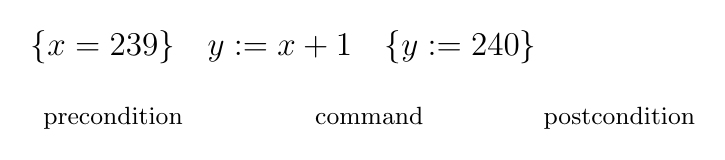
\begin{tikzpicture}[x=0.75pt,y=0.75pt,yscale=-1,xscale=1]


% Text Node
\draw (223,30) node [anchor=north west][inner sep=0.75pt]  [font=\large]  {$\textcolor[rgb]{0,0,0}{\{x = 239\}} \ \ \ y := x + 1\ \ \ \{y := 240\}$};
% Text Node
\draw (229,67) node [anchor=north west][inner sep=0.75pt]  [font=\small] [align=left] {precondition};
% Text Node
\draw (360,67) node [anchor=north west][inner sep=0.75pt]  [font=\small] [align=left] {command};
% Text Node
\draw (470,67) node [anchor=north west][inner sep=0.75pt]  [font=\small] [align=left] {postcondition};


\end{tikzpicture}
  \end{center}
  \vspace*{-70pt}
\end{figure}
Basically, the Hoare triple is statement, which denotes that
% Украдено с википедии.
when the precondition is met, executing the command establishes the postcondition. 
To construct new triples and assertions, Hoare Logic introduces \textit{inference rules}, which take the form as shown in Figure~\ref{fig:hoare_rule}.
\begin{figure}[H]
  \vspace*{-15pt}
  \begin{center}
    \tikzset{every picture/.style={line width=0.75pt}} %set default line width to 0.75pt        

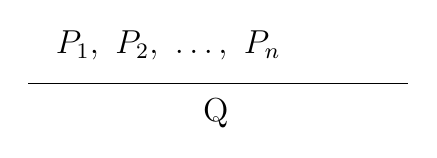
\begin{tikzpicture}[x=0.75pt,y=0.75pt,yscale=-1,xscale=1]
%uncomment if require: \path (0,104); %set diagram left start at 0, and has height of 104

%Straight Lines [id:da3574993852788938] 
\draw    (238,57) -- (421,57) ;

% Text Node
\draw (250,30.4) node [anchor=north west][inner sep=0.75pt]  [font=\large]  {$P_{1} ,\ P_{2} ,\ \dotsc ,\ P_{n}$};
% Text Node
\draw (321,63) node [anchor=north west][inner sep=0.75pt]  [font=\large] [align=left] {Q};


\end{tikzpicture}

  \end{center}
  \vspace*{-60pt}
  \caption{Hoare rule notation}
  \label{fig:hoare_rule}
\end{figure}
The inference rules assert the following: if all the \textit{premises} $P_1, P_2, \dotsc, P_n$ are satisfied, then the \textit{conclusion} $Q$ is also satisfied.
In addition to the ability to create custom rules (provided that their correctness is proved), Hoare Logic includes a set of standard rules --- \textit{axioms}.
\begin{figure}[H]
  \vspace*{-15pt}
  \begin{center}
    \tikzset{every picture/.style={line width=0.75pt}} %set default line width to 0.75pt        

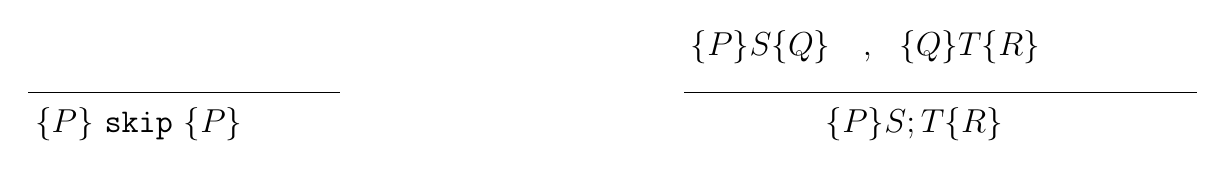
\begin{tikzpicture}[x=0.75pt,y=0.75pt,yscale=-1,xscale=1]
%uncomment if require: \path (0,104); %set diagram left start at 0, and has height of 104

%Straight Lines [id:da43085718847463716] 
\draw    (92,53) -- (242,53) ;
%Straight Lines [id:da073972515186154] 
\draw    (408,53) -- (655,53) ;

% Text Node
\draw (410,22) node [anchor=north west][inner sep=0.75pt]  [font=\large]  {$\{P\} S\{Q\} \ \ \ ,\ \ \{Q\} T\{R\}$};
% Text Node
\draw (94, 59) node [anchor=north west][inner sep=0.75pt]  [font=\large]  {$\{P\} \ \mathtt{skip} \ \{P\}$};
% Text Node
\draw (475,59) node [anchor=north west][inner sep=0.75pt]  [font=\large]  {$\{P\} S;T\{R\}$};


\end{tikzpicture}

  \end{center}
  \vspace*{-50pt}
  \caption[fontsize=\small]{Hoare axiom rules examples}
\end{figure}

However, despite the fact that Hoare Logic is a highly potent tool for working with imperative programming languages, 
it has a number of limitations. The biggest one is the lack of support for pointers, 
which is especially relevant for reasoning about imperative programs. To address this problem, 
Hoare Logic was extended to Separation Logic by John C. Reynolds and Peter O'Hearn in 2002~\cite{reynolds}. 
It allows for working with statements of the form $s, h \models P$, where $s$ is a store, $h$ is a heap and 
$P$ is an assertion over the given store and heap.
Separation Logic also introduces several new constants and operators that allow for constructing
statements related to memory. We will consider only those that are relevant for our work:
\begin{itemize}
  % Wikipedia
  \item Constant \textbf{emp} --- constant, which asserts that heap is empty. For instance
  $s, h \models \bf{emp}$ when $h$ is undefined for all adresses.
  \item Operator $e \mapsto e'$ denotes that heap is defined at address $e$ and contains value $e'$.
  \item Operator $s, h \models P * Q$ denotes that there exist $h_1, h_2$ such
  and $h = h_1 \sqcup h_2$ and $s, h_1 \models P$ and $s, h_2 \models Q$.
\end{itemize}

\subsubsection{Verified Software Toolchain(VST)}
Currently, formal verification of programs is only possible for programs written in C. 
The commonly accepted approach is to use two tools: 
\begin{itemize}
  \item The \textbf{CompCert \textit{clightgen} tool} is part of the formally verified C compiler CompCert, 
  which allows translating C code into its representation as an AST in Coq.
  \item The \textbf{Verified Software Toolchain(VST)} is a Coq framework for verifying C programs, compiled by CompCert.
  Particulary, we will be interested in \textbf{VST-Floyd} library for Coq, that provides a set of tactics and lemmas for reasoning about C programs.
\end{itemize}

\section{Implementation of the library in C}
In this section, we will provide a brief overview of the implementation of our C library, 
examine examples of the most important functions, 
and also discuss the solutions we have adopted due 
to the use of an imperative programming language (as well as to simplify verification).

\subsection{\texttt{Format} representation}
As shown in the Figure~\ref{fig:format}, the \texttt{Format} structure consists of 5 fields. \texttt{height},
\texttt{first\_line\_width}, \texttt{middle\_width}, \texttt{last\_line\_width} are
natural numbers and thus can be represented as \texttt{unsigned int}(which is done in our implementation).
However, the \texttt{to\_text} field is a function and in general can't be conveniently represented in C, so
we had to turn to the semantics of this function.

We noticed that the shift and line parameters in the original functional library exist solely for the sake of code simplicity and
are not an essential part of the algorithm. 
It is easy to see that given a Format \texttt{G}, 
a natural number \texttt{shift}, and a string \texttt{line}, we can recover \texttt{G.to\_text(shift, line)}
from just \texttt{G.to\_text(0, EmptyString)}. Therefore, we made the decision to store a linked list of strings instead of the \texttt{to\_text} function. 
\begin{figure}[H]
\begin{minipage}{0.5\textwidth}
\definecolor{bg}{rgb}{0.95,0.95,0.95}

\begin{mdframed}[backgroundcolor=bg]
\begin{minted}[fontsize=\small]{cpp}
struct format {
  unsigned int height;
  unsigned int first_line_width;
  unsigned int middle_width;
  unsigned int last_line_width;
  list *to_text;
} typedef format;
\end{minted}
\end{mdframed}
\vspace*{-35pt}
\end{minipage}
\begin{minipage}{0.5\textwidth}
\definecolor{bg}{rgb}{0.95,0.95,0.95}

\begin{mdframed}[backgroundcolor=bg]
\begin{minted}[fontsize=\small]{cpp}
struct list {
  size_t shift;
  char *line;
  struct list *tail;
} typedef list;
\end{minted}
\end{mdframed}
\end{minipage}
\vspace*{30pt}
\caption{\texttt{Format} in C}
\label{fig:format_C}
\end{figure}
Additionally, the string indendation and concatenation functions were made independent of the \texttt{Format} structure.
Implementations of \texttt{Format} structure and linked list are shown in Figure~\ref{fig:format_C}.

In our implementation, each combinator returns a completely new Format that is not a reference to any other Format, 
as each Format can be reused many times during the algorithm. And since sometimes the result of a combinator work 
is equal to one of the Formats passed to it, it is necessary to have function, that creates a copy of a specific Format. 
Thus, the main functions for manipulating Formats, in addition to printer-combinator functions, are
\texttt{format\_copy} and \texttt{list\_copy}, which turned out to be one of the most difficult function to verify in the first part of the work.
\begin{figure}[H]
\begin{minipage}{0.55\textwidth}
\definecolor{bg}{rgb}{0.95,0.95,0.95}

\begin{mdframed}[backgroundcolor=bg]
\begin{minted}[fontsize=\small]{cpp}
list *list_copy(list *l) {
  if (l == NULL) return NULL;
  list *new = malloc(sizeof(list));
  if(!new) exit(1);

  list *cur = new;
  list *l_cur = l;
  while(true) {
    cur->shift = l_cur->shift;
    cur->line =
       malloc(strlen(l_cur->line) + 1);
    if(!cur->line) exit(1);
    strcpy(cur->line, l_cur->line);
    cur->tail = NULL;

    if (l_cur->tail == NULL) {
      cur = NULL;
      break;
    }
    cur->tail =
       malloc(sizeof(list));
    if(!cur->tail) exit(1);
    cur = cur->tail;
    l_cur = l_cur->tail;
  }
  return new;
}
\end{minted}
\end{mdframed}
\vspace*{-210pt}
\end{minipage}
\begin{minipage}{0.46\textwidth}
\definecolor{bg}{rgb}{0.95,0.95,0.95}

\begin{mdframed}[backgroundcolor=bg]
\begin{minted}[fontsize=\small]{cpp}
format* format_copy(format *G) {
  format* result =
       malloc(sizeof(format));
  if(!result) exit(1);
  result->height = G->height;
  result->first_line_width = 
      G->first_line_width;
  result->middle_width = 
      G->middle_width;
  result->last_line_width = 
      G->last_line_width;
  result->to_text =
       list_copy(G->to_text);
  return result;
}
\end{minted}
\end{mdframed}
\end{minipage}
\vspace*{210pt}
\caption{\texttt{list\_copy} and \texttt{format\_copy} functions}
\label{fig:format_copy}
\end{figure}
Our implementations of \texttt{list\_copy} and \texttt{format\_copy} function are shown in Figure~\ref{fig:format_copy}.
Note that the importance of implementing and verifying these functions will be particularly noticeable in the future sections
when discussing the internal structure of the functions that implement printer combinators.

\subsection{Standard library}
Since our library is heavily focused on working with text, basic functions from the standard library, 
in particular from \texttt{string.h}, are required for manipulating our Formats. However, 
in VST-Floyd, only the functions \texttt{malloc}, \texttt{free}, and \texttt{exit} were verified. 
Therefore, all the necessary functions we wanted had to be implemented from scratch. In total, we used 3 functions 
from standard library, let's take a closer look at each one of them:

\begin{enumerate}
  \item \texttt{strlen} --- function that returns the length of the string. 
    The implementation of this function is shown in Figure~\ref{fig:strlen}.
      \begin{figure}[H]
      \definecolor{bg}{rgb}{0.95,0.95,0.95}

      \begin{mdframed}[backgroundcolor=bg]
      \begin{minted}[fontsize=\small]{cpp}
size_t strlen(const char *str) {
  size_t i;
  for (i=0; ; i++)
    if (str[i]==0) 
      return i;
}
      \end{minted}
      \end{mdframed}
      \caption{\texttt{strlen} implementation}
      \label{fig:strlen}
      \end{figure}
    The function takes a pointer to the string and iterates over it until it finds a null character. 
    Then it returns the number of characters that have been iterated over. In our library it mostly used to
    calculate number of bits to then put it to the \texttt{malloc} function.
  \item \texttt{strcpy} --- function that copies the string pointed to by \texttt{src} to the buffer pointed to by \texttt{dest}. 
    The implementation of this function is shown in Figure~\ref{fig:strcpy}.
      \begin{figure}[H]
      \definecolor{bg}{rgb}{0.95,0.95,0.95}
      \begin{mdframed}[backgroundcolor=bg]
      \begin{minted}[fontsize=\small]{cpp}
char *strcpy(char *dest, const char *src) {
  size_t i;
  for(i = 0;; i++){
    char d = src[i];
    dest[i] = d;
    if(d == 0) return dest;
  }
}
      \end{minted}
      \end{mdframed}
      \caption{\texttt{strcpy} implementation}
      \label{fig:strcpy}
      \end{figure}
    The function takes two pointers to the strings and iterates over the first one until it finds a null character. 
    Then it copies the characters from the first string to the second one. 
    In our library it is used only once --- in the function that copies the \texttt{Format} structure.
  \item \texttt{strcat} --- function that concatenates the string pointed to by \texttt{src} to the end of the string pointed to by \texttt{dest}.
    The implementation of this function is shown in Figure~\ref{fig:strcat}.
      \begin{figure}[H]
      \definecolor{bg}{rgb}{0.95,0.95,0.95}
      \begin{mdframed}[backgroundcolor=bg]
      \begin{minted}[fontsize=\small]{cpp}
char *strcat(char *dest, const char *src) {
  size_t i,j;
  for(i = 0;;i++){
    char d = dest[i];
    if(d == 0) break;
  }
  for(j = 0;;j++){
    char d = src[j];
    dest[i + j] = d;
    if(d == 0) return dest;
  }
}
      \end{minted}
      \end{mdframed}
      \caption{\texttt{strcat} implementation}
      \label{fig:strcat}
      \end{figure}
    The function takes two pointers to the strings and iterates over the first one until it finds a null character. 
    Then it iterates over the second string and copies the characters to the first one.
    In our library it is used in \texttt{add\_beside} and \texttt{add\_fill} combinators, as they take two
    Formats as argumants and concatenate the last string of the first Format and the first string of the second Format.
\end{enumerate}
Another function that is not included in the standard C library, but which we deemed appropriate to add to this section, is the \texttt{max} function.
      \begin{figure}[H]
      \definecolor{bg}{rgb}{0.95,0.95,0.95}
      \begin{mdframed}[backgroundcolor=bg]
      \begin{minted}[fontsize=\small]{cpp}
unsigned int max(unsigned int a, unsigned int b) {
  if (a <= b)
    return b;
  return a;
}
      \end{minted}
      \end{mdframed}
      \caption{\texttt{max} implementation}
      \label{fig:max}
      \end{figure}
  The \texttt{max} function is used 17 times in our library and is used to calculate new dimensions in all combinators, 
  so its implementation and verification were necessary for the readability of our library code.

\newpage
\subsection{Combinators representation}
Let's examine in detail the internal structure of printer combinators in our reference library.
\begin{figure}[H]
\definecolor{bg}{rgb}{0.95,0.95,0.95}
\begin{mdframed}[backgroundcolor=bg]
\begin{minted}[fontsize=\small]{coq}
Definition add_beside (G:t) (G':t):t :=
match G.(height), G'.(height) with
  | O, _ => G'
  | _, O => G
  | _, _ => 
    let middle_width_new :=
       match G.(height), G'.(height) with
       | 1,(1|2) => G.(first_line_width) + G'.(first_line_width)
       | _,1     => G.(middle_width)
       | 1,_     => G.(last_line_width) + G'.(middle_width)
       | 2,_     => max (G.(last_line_width) + G'.(first_line_width))
                        (G.(last_line_width) + G'.(middle_width))
       | _,_     => max G.(middle_width)
                    (max (G.(last_line_width) + G'.(first_line_width))
                         (G.(last_line_width) + G'.(middle_width)))
       end
    in
      let first_line_width_new :=
         if (G.(height) =? 1) then 
            G.(first_line_width) + G'.(first_line_width) 
         else
            G.(first_line_width)
      in
         T
          (G.(height) + G'.(height) - 1)
          first_line_width_new
          middle_width_new 
          (G.(last_line_width) + G'.(last_line_width))
          (fun s t => 
            G.(to_text) s (G'.(to_text) (s + G.(last_line_width)) t))
end.
\end{minted}
\end{mdframed}
\caption{\texttt{add\_beside} combinator in functional library}
\label{fig:add_beside_coq}
\end{figure}

As you can see in Figure~\ref{fig:add_beside_coq}, the \texttt{add\_beside} combinator (as well as any other combinator, in general) 
consists of several more or less independent parts. In our C implementation of the library, we tried to move as many calculations as possible 
out of the main combinator function to make the code more concise and easier to verify. Let's go through each part of the combinator in more detail:
\begin{enumerate}
  \item \textbf{Beginning of the combinator}. It's easy to see (and it's actually verified in our library), that height of a Format equals to zero if and only if
  the Format doesn't contain any text (i.e. our C list is empty). In that case, whenever one of the arguments of combinator has height
  equal to zero, the second argument will be result of our combinator. 
\begin{figure}[H]
\definecolor{bg}{rgb}{0.95,0.95,0.95}
\begin{mdframed}[backgroundcolor=bg]
\begin{minted}[fontsize=\small]{cpp}
format *add_beside(format *G, format *F) {
  if (G->height == 0) {
    return format_copy(F);
  } 
  if (F->height == 0) {
    return format_copy(G);
  }

  t* result = malloc(sizeof(format));
  if(!result) exit(1);
\end{minted}
\end{mdframed}
\caption{Beginning of \texttt{add\_beside} function in C}
\label{fig:zero_height_check}
\end{figure}

  In our library, this logic is supported by relatively simple conditions
  as shown in Figure~\ref{fig:zero_height_check}.
  Moreover, because this reasoning apply to all combinators at once, this piece of code appears in all functions: \texttt{add\_above}, \texttt{add\_beside}, and \texttt{add\_fill}. 
  It is also worth noting that it is exactly at this point that we need \texttt{format\_copy}, because without it, 
  we would have to return a pointer to one of the arguments, which obviously does not suit us due to the multiple reuse of the same Format in different combinators.

  \item \textbf{Format height calculation}. As shown in Figure~\ref{fig:add_beside_coq}, the height of the resulting Format is calculated 
  in a pretty straightforward way without any case distinction.
  In fact, a similar formula is applicable to almost all combinators (except that in \texttt{add\_above} the height is equal to \texttt{G.height + G'.height}). 
\begin{figure}[H]
\definecolor{bg}{rgb}{0.95,0.95,0.95}
\begin{mdframed}[backgroundcolor=bg]
\begin{minted}[fontsize=\small]{cpp}
result->height = G->height + F->height - 1;
\end{minted}
\end{mdframed}
\caption{Height calculation in \texttt{add\_beside} function in C}
\label{fig:height_calculation}
\end{figure}
  Thus, in all combinators, the height calculation always corresponds to only one line, and in the case of \texttt{add\_beside}, this line is shown in Figure~\ref{fig:height_calculation}.

  \item \textbf{Format first line width calculation}. Here is where the differences between the combinators begin. 
  Obviously, in \texttt{add\_above}, the first line width is always equal to the first line width of the first argument (if it is not empty). 
  However, in \texttt{add\_beside} and \texttt{add\_fill}, the situation may be different if the height of the first argument is one. 
  In this case, the first line widths of both arguments are added together.
\begin{figure}[H]
\definecolor{bg}{rgb}{0.95,0.95,0.95}
\begin{mdframed}[backgroundcolor=bg]
\begin{minted}[fontsize=\small]{cpp}
unsigned int flw_add_beside(format *G, format *F) {
  if(G->height == 0)
    return F->first_line_width;
  if(F->height == 0)
    return G->first_line_width;

  unsigned int first_line_width_new;
  if (G->height == 1)
    first_line_width_new = G->first_line_width + F->first_line_width;
  else
    first_line_width_new = G->first_line_width;
  return first_line_width_new;
}
\end{minted}
\end{mdframed}
\caption{\texttt{add\_beside} first line width calculation in C}
\label{fig:flw_calculation}
\end{figure}
  Now, there is a case distinction and the logic is no longer primitive. For ease of verification we put this piece of code into a separate function, as shown in Figure~\ref{fig:flw_calculation}.

  \item \textbf{Middle width calculation}.
  Now the formulas become slightly more complicated, because the value of middle line width itself has a rather complex semantics. 
  In the case when the Format height is equal to one, middle line width is equal to the width of the only line in the Format. 
  In the case when the Format height is equal to two, middle line width is equal to the first line width of this Format. 
  In all other cases, middle line width is equal to the maximum width of all the lines located between the first and last lines in the Format.
\begin{figure}[H]
\definecolor{bg}{rgb}{0.95,0.95,0.95}
\begin{mdframed}[backgroundcolor=bg]
\begin{minted}[fontsize=\small]{cpp}
unsigned int mdw_add_beside(format *G, format *F) {
  if(G->height == 0)
    return F->middle_width;
  if(F->height == 0)
    return G->middle_width;

  unsigned int middle_width_new;
  if (G->height == 1 && F->height == 1) {
    middle_width_new = G->first_line_width + F->first_line_width;
  } else if(G->height == 1 && F->height == 2) {
    middle_width_new = G->first_line_width + F->first_line_width;
  } else if (F->height == 1) {
    middle_width_new = G->middle_width;
  } else if (G->height == 1) {
    middle_width_new = G->last_line_width + F->middle_width;
  } else if (G->height == 2) {
    middle_width_new = max(G->last_line_width + F->first_line_width, 
                            G->last_line_width + F->middle_width);
  } else {
    middle_width_new = max(G->middle_width,
                          max(G->last_line_width + F->first_line_width, 
                              G->last_line_width + F->middle_width));
  }
  return middle_width_new;
}
\end{minted}
\end{mdframed}
\caption{\texttt{add\_beside} middle line width calculation in C}
\label{fig:mlw_calculation}
\end{figure}
As shown in Figure~\ref{fig:mlw_calculation}, the middle line width for the \texttt{add\_beside} combinator is calculated in a rather cumbersome way. 
Due to the reasons described above, for other Formats the size of the formula remains more or less the same (although its content may change).

  \item \textbf{Format last line width calculation}. The situation is very similar to the calculation of height.
  In two out of three combinators (\texttt{add\_above} and \texttt{add\_beside}), the calculation is done in one line of code.
\begin{figure}[H]
\definecolor{bg}{rgb}{0.95,0.95,0.95}
\begin{mdframed}[backgroundcolor=bg]
\begin{minted}[fontsize=\small]{cpp}
result->last_line_width = G->last_line_width + F->last_line_width;
\end{minted}
\end{mdframed}
\caption{\texttt{add\_beside} last line width calculation in C}
\label{fig:llw_calculation}
\end{figure}

  \item \textbf{Format to\_text calculating}. This part is the most non-trivial of all. 
  There are no formulas here, however, we need to build a complex structure, shown in Figure~\ref{fig:combinators}. 

\begin{figure}[H]
\definecolor{bg}{rgb}{0.95,0.95,0.95}
\begin{mdframed}[backgroundcolor=bg]
\begin{minted}[fontsize=\small]{cpp}
list *to_text_add_beside(format *G, format *F) {
  if(G->height == 0)
    return list_copy(F->to_text);
  if (F->height == 0)
    return list_copy(G->to_text);
  list *head = list_copy(G->to_text);                        /* a */
  list *tail = get_list_tail(head);                          /* b */
  list *copy_F = list_copy(F->to_text);                      /* a */
  tail->line = 
    line_concats(tail->line, copy_F->shift, copy_F->line);   /* c */
  shift_list(copy_F->tail, G->last_line_width);              /* d */
  tail->tail = copy_F->tail;                                 /* e */
  free(copy_F);                                              /* f */
  return head;
}
\end{minted}
\end{mdframed}
\caption{\texttt{add\_beside} \texttt{to\_text} calculation in C}
\label{fig:to_text_calculation}
\end{figure}

  Let's break down the steps of the algorithm that might work for us:
  \begin{enumerate}
    \item Copy Formats G and F.
    \item Find the tail of Format G. \textit{We explicitly write this as a separate step, as it is a non-trivial task in a singly linked list.}
    \item Concatenate a string from the tail of Format G with the first line of Format F.
    \item Shift all lines of Format F, starting from the second,\newline by \texttt{G.last\_line\_width}.
    \item Connect the modified G and the modified F starting from the second line.
    \item Free the remaining unused data.
  \end{enumerate}
  And exactly this algorithm we implemented in our library. Its correctness was also proven, although we will talk about it in the next chapter.
  % Дописать про get_list_tail, line_concats, shift_list
\end{enumerate}

Thus, it remains to put it all together in the function shown in Figure~\ref{fig:add_beside_C}.
\begin{figure}[H]
\definecolor{bg}{rgb}{0.95,0.95,0.95}
\begin{mdframed}[backgroundcolor=bg]
\begin{minted}[fontsize=\small]{cpp}
format *add_beside(format *G, format *F) {
  if (G->height == 0) return format_copy(F);
  if (F->height == 0) return format_copy(G);
  format* result = malloc(sizeof(format));
  if(!result) exit(1);

  unsigned int middle_width_new = mdw_add_beside(G, F);
  unsigned int first_line_width_new = flw_add_beside(G, F);
  list *to_text_new = to_text_add_beside(G, F);

  result->height = G->height + F->height - 1;
  result->first_line_width = first_line_width_new;
  result->middle_width = middle_width_new;
  result->last_line_width = 
    G->last_line_width + F->last_line_width;
  result->to_text = to_text_new;
  return result;
}
\end{minted}
\end{mdframed}
\caption{\texttt{add\_beside} implementation in C}
\label{fig:add_beside_C}
\end{figure}

In fact, after writing a function for constructing \texttt{to\_text} in \texttt{add\_beside}, the other combinators will not cause any particular problems. 
It is easy to see that by replacing \texttt{G.last\_line\_width} with an arbitrary shift in the algorithm, we get \texttt{add\_fill}. 
Moreover, to construct the list for \texttt{add\_above}, it is only necessary to concatenate \texttt{G.to\_text} and \texttt{F.to\_text}, which is done trivially, having the \texttt{get\_list\_tail} function.

\subsection{Implementation of lists functions}
During the traversal of the \texttt{Doc} structure, our algorithm examines the type of node it is currently in and processes the lists 
(or a single list in the case of \texttt{Indent} node) obtained from its children in one way or another. 
This section will cover the implementation of the functions used for this purpose.

\begin{figure}[H]
\definecolor{bg}{rgb}{0.95,0.95,0.95}
\begin{mdframed}[backgroundcolor=bg]
\begin{minted}[fontsize=\small]{coq}
Definition cross_general (width: nat) (op: t -> t -> t) 
                          (fl1: list t) (fl2: list t) :=
  List.filter (fun f => total_width f <=? width)
    (List.concat (map (fun b => map (fun a => op a b) fl1) fl2)).

Definition constructDoc (s: string) := (of_string s)::nil.

Definition indentDoc (width: nat) (shift: nat) (fs: list t) :=
  cross_general width (fun _ b => indent' shift b) (empty::nil) fs.

Definition besideDoc (width: nat) (fs1: list t) (fs2: list t) := 
  cross_general width add_beside fs1 fs2.

Definition aboveDoc (width: nat) (fs1: list t) (fs2: list t) := 
   cross_general width add_above fs1 fs2.

Definition fillDoc (width: nat) (fs1: list t) 
                    (fs2: list t) (shift: nat) :=
   cross_general width (fun fs f => add_fill fs f shift) fs1 fs2.

Definition choiceDoc (fs1: list t) (fs2: list t) := 
    fs1 ++ fs2.
\end{minted}
\end{mdframed}
\caption{\texttt{Doc} functions in reference library}
\label{fig:doc_functions}
\end{figure}

The figure~\ref{fig:doc_functions} shows a rather concise implementation of \texttt{Doc} functions (that's how we will call functions operating on \texttt{Doc} nodes) from the reference library. 
All functions, except for \texttt{constructDoc}, use \texttt{cross\_general} in their implementation, which takes the global parameter \texttt{w}, limiting the maximum width of the Format, the function \texttt{op}, which will be applied to all pairs of Formats from two lists, 
and two lists of Formats. It is easy to see that semantically this function is a generalization of pairwise application of combinators to two lists, nevertheless, the authors of the library also used it to implement \texttt{indentDoc}, replacing one of the lists with a list consisting of one element 
and passing a function ignoring one of the lists and shifting the second list by \texttt{shift} as an \texttt{op} argument.
It is also important to note that the \texttt{cross\_general} function automatically removes Formats whose width exceeds \texttt{w}, which allows us to obtain a list of Formats whose width does not exceed \texttt{w} as a result of the algorithm's work.

Due to the complexity of working with templates and function pointers in verifying C programs, we decided to abandon such an approach and implemented 6 independent functions. 
Let's consider their implementation using the example of \texttt{besideDoc}. We'll go through the code of this function step by step:
\begin{enumerate}
  \item One of the most important parts of writing verified programs is checking for \texttt{NULL} pointers in case there are no guarantees. 
  In our case, each of the \texttt{Doc} functions frees the memory of the lists passed to it as arguments. 
  This was done because during the descent through the \texttt{Doc} structure, reusing the same list never happens, in other words, the list stops being available as soon as the algorithm exits the current node of the tree. 
  And since memory must be freed for correctness of the program, it was decided to incorporate this logic into the \texttt{Doc} functions, thus making them full-fledged for handling corresponding types of nodes.
\begin{figure}[H]
\definecolor{bg}{rgb}{0.95,0.95,0.95}
\begin{mdframed}[backgroundcolor=bg]
\begin{minted}[fontsize=\small]{cpp}
if (fs1 == NULL) {
  if (fs2 != NULL)
    clear_format_list(fs2);
  return NULL;
}
if (fs2 == NULL) {
  clear_format_list(fs1);
  return NULL;
}
\end{minted}
\end{mdframed}
\caption{NULL check in \texttt{besideDoc}}
\label{fig:beside_doc_null_check}
\end{figure}

  \item Next, in Figure~\ref{fig:beside_doc_initialization}, you can see the initialization of the main variables that we will use throughout this function. 
\begin{figure}[H]
\definecolor{bg}{rgb}{0.95,0.95,0.95}
\begin{mdframed}[backgroundcolor=bg]
\begin{minted}[fontsize=\small]{cpp}
  format_list *result = malloc(sizeof(format_list));
  if(result == NULL) exit(1);
  result->G = empty();
  result->tail = NULL;
  format_list *result_tail = result;
  bool has_item = false;
\end{minted}
\end{mdframed}
\caption{Initialization in \texttt{besideDoc}}
\label{fig:beside_doc_initialization}
\end{figure}
  We would like to highlight two points:
  \begin{itemize}
    \item Firstly, the use of the variable \texttt{has\_item}, which becomes true when an element is added to our resulting list \texttt{result}. 
    If \texttt{has\_item} remains false, it means that no element has been added to our list, and the pointer \texttt{result} can be freed.
    \item Secondly, the initialization of the Format in the head of the list with an empty Format was done to maintain the invariant of the \texttt{result} array --- 
    the first elements are the elements obtained as a result of the combinators work, and the last element is always equal to \texttt{empty}. Otherwise, the last format would always remain uninitialized, 
    and the description of the invariant would become much more complicated.
  \end{itemize}

\item In the Figure~\ref{fig:beside_doc_main} you can see the main part of the function, that replaces the \texttt{cross\_general} function, perfoming pairwise application of combinators and filtering the results by width and height 
(in the reference library, there is no filtering by height, its appearance will be discussed in detail in Chapter~\ref{chapter_verification}).
\begin{figure}[H]
\definecolor{bg}{rgb}{0.95,0.95,0.95}
\begin{mdframed}[backgroundcolor=bg]
\begin{minted}[fontsize=\small]{cpp}
format_list *fs2_tail = fs2;
while(fs2_tail != NULL) {
  format_list *fs1_tail = fs1;
  while(fs1_tail != NULL) {
    t* G = add_beside(fs1_tail->G, fs2_tail->G);
    if(max_width_check(G, width, height)) {
      clear_to_text(result_tail->G->to_text);
      free(result_tail->G);
      result_tail->G = G;
      result_tail->tail = malloc(sizeof(format_list));
      if(result_tail->tail == NULL) exit(1);
      result_tail->tail->G = empty();
      result_tail->tail->tail = NULL;
      result_tail = result_tail->tail;
      has_item = true;
    } else {
      clear_to_text(G->to_text);
      free(G);
    }
    fs1_tail = fs1_tail->tail;
  }
  fs2_tail = fs2_tail->tail;
}
\end{minted}
\end{mdframed}
\caption{Main part in \texttt{besideDoc}}
\label{fig:beside_doc_main}
\end{figure}

\item The last part of the function is responsible for freeing up memory, in particular, deleting the empty Format written at the end of the \texttt{result} array, 
as well as deleting the entire list if \texttt{has\_item} is false.
\begin{figure}[H]
\definecolor{bg}{rgb}{0.95,0.95,0.95}
\begin{mdframed}[backgroundcolor=bg]
\begin{minted}[fontsize=\small]{cpp}
  clear_format_list(fs1);
  clear_format_list(fs2);
  if(!has_item) {
    clear_format_list(result);
    return NULL;
  }
  format_list *new_result_tail = result;
  while(new_result_tail->tail->tail != NULL) {
    new_result_tail = new_result_tail->tail;
  }
  clear_format_list(new_result_tail->tail);
  new_result_tail->tail = NULL;
  return result;
\end{minted}
\end{mdframed}
\caption{Final part in \texttt{besideDoc}}
\label{fig:beside_doc_free}
\end{figure}
\end{enumerate}

\texttt{aboveDoc} and \texttt{fillDoc} are implemented in a similar way (the only difference is which combinator is used in the main part), 
while \texttt{indentDoc} and \texttt{choiceDoc} have a fairly straightforward implementation, partially reusing previously written functions.

\label{chapter_verification}
\section{Verification of the pretty-printing library}
In section~\ref{detailed_description_of_the_algorithm} we discussed the algorithm, that is 
goint to give us a list of Formats that satisfy certain conditions. Thus, the highest-level part of our algorithm is the function that performs a descent through the tree and recursively processes lists of Formats.
This function, depending on the type of the current node, processes the received lists of Formats in various ways, recursively. 
Each such operation is represented as a separate function that takes two lists of Formats and creates a new one based on the arguments. 
There are 5 such functions in total --- \texttt{identDoc}, \texttt{choiceDoc}, \texttt{besideDoc}, \texttt{aboveDoc}, and \texttt{fillDoc} 
(we have described in more detail how each of them works earlier in section~\ref{detailed_description_of_the_algorithm}). 
Because all these functions use Formats that are the results of the work of these same functions, there must be an invariant under which all Formats that interact with these functions must fit. 
In this chapter we will discuss the limitations that must be imposed on Formats, as well as the intermediate steps that had to be taken to satisfy these limitations.

\subsection{Overflow problems}
As our algorithm is entirely based on a functional library, the issue of Format characteristics overflow was not considered. 
To address the problem in our case, we decided to impose constraints on the Formats passed to the functions for working with lists.
\begin{itemize}
  \item First of all, there is a restriction on the height of the Format. 
  The original algorithm takes height as a parameter, by which we filter our Formats, but does not impose any restrictions on it. 
  In our implementation, the restriction $0 \le 2 \cdot \text{\texttt{max\_height}} \le \text{\texttt{Int.max\_unsigned}}$ is applied. 
  The constant 2 appears because the height of the Format increases no more than 2 times as a result of the combinator's operation
  (moreover, in the \texttt{add\_above} combinator, it increases exactly by a factor of 2), 
  and we must always be within the limits of the \texttt{unsigned int} data type to avoid overflow and data loss.
  \item Secondly, the width of the Format also plays an important role and has the ability to increase indefinitely as a result of the combinators' operations. 
  In the reference library, the width is not a global parameter of the algorithm, however, in our implementation, it was introduced to control the growth of the corresponding Format characteristics 
  (of course, such a modification also allowed for more flexible description of the list of Formats we want to obtain). 
  This parameter received similar restrictions to height --- $0 \le 2 \cdot \text{\texttt{max\_width}} \le \text{\texttt{Int.max\_unsigned}}$, because by default, 
  the width can increase by this factor as a result of the combinator's operation.
  \item Of course, limitations on the width of the Format do not fully solve the problem of overflow, since it is still possible to pass an arbitrary number to the \texttt{shiftDoc} function. 
  To address this problem, we impose a restriction on the \texttt{shift} parameter passed to \texttt{shiftDoc} and \texttt{indentDoc}. 
  The restriction will be of the form $0 \le \text{\texttt{shift}} \le \text{\texttt{max\_width}}$, since in each line, the width becomes either the sum of the widths of the two Format lines or the width of one of the Format lines plus \texttt{shift}. 
  In each of these cases, when the above restriction is met, and the width of each Format line does not exceed \texttt{max\_width}, we always remain within the boundaries of \texttt{unsigned int} and overflow does not occur.
\end{itemize}

Let's call a Format \textit{good} if its height does not exceed \texttt{max\_height} and its width (the maximum of \texttt{first\_line\_width}, \texttt{middle\_width}, and \texttt{last\_}\texttt{line\_}\newline\texttt{width}) does not exceed \texttt{max\_width}. 
As we have shown earlier, by passing good Formats to the \texttt{aboveDoc}, \texttt{besideDoc}, and \texttt{fillDoc} functions, there will be no overflows as a result of the combinators' work inside these functions.
Of course, these constraints should be an invariant of the Formats when working with lists due to the constant use of these Formats in recursive calls. 
Therefore, in the functions \texttt{aboveDoc}, \texttt{besideDoc}, and \texttt{fillDoc}, we explicitly check the result of each combinator for compliance with our constraints and discard the Format if the constraints were not satisfied.

Since the functions implementing the work of the printer combinators can be used in an extended version of the library, 
in algorithms without global parameters \texttt{max\_width} and \texttt{max\_height}, we want to avoid using this parameter when specifying the requirements necessary for the function to work correctly. 
At the same time, of course, we still want to avoid overflows, which in our case lead to data loss. The constraint we will impose on one of the arguments \texttt{G} will be quite straightforward:
\begin{enumerate}
  \item $0 \le 2 \cdot \texttt{G.height} \le \texttt{Int.max\_unsigned}$
  \item $\forall (\texttt{ident}, \texttt{line}) \in \texttt{G.to\_text}:\\ 0 \le 2 \cdot (\texttt{ident} + \texttt{length(line)}) \le \texttt{Int.max\_unsigned}$
  \item $0 \le 2 \cdot \texttt{shift} \le \texttt{Int.max\_unsigned}$ --- in case of \texttt{add\_fill} combinator.
\end{enumerate}

It is easy to see that if two combinators satisfy the above constraints, then overflow of Format characteristics cannot occur.
In this case, we assume that the user will not need to create Formats with dimensions on the order of billions of characters.

\subsection{Correctness of Format \texttt{to\_text} C respresentation}
One of the obvious problems that arise in our approach with a list of strings is the absence of a similar structure in the reference library. 
As a result, there is no object with which our list could be linked, and therefore all its properties and its relation to Format characteristics must be proved independently.

To address this issue, we have introduced a list of properties that we will call \textit{basic} and which will be an invariant when working with Formats in all functions in which they participate 
(including combinators and functions for working with lists).
\begin{itemize}
  \item Constraints on all Format characteristics. 
  They need to be explicitly defined so that regardless of the existence of constraints in a particular function, our \texttt{Format} structure always makes sense:
  \begin{enumerate}
    \item $0 \le \texttt{G.height} \le \texttt{Int.max\_unsigned}$
    \item $0 \le \texttt{G.first\_line\_width} \le \texttt{Int.max\_unsigned}$
    \item $0 \le \texttt{G.middle\_width} \le \texttt{Int.max\_unsigned}$
    \item $0 \le \texttt{G.last\_line\_width} \le \texttt{Int.max\_unsigned}$
  \end{enumerate}
  \item Similarly, there must be constraints on the \texttt{to\_text} list belonging to each Format, since in our implementation, 
  each Format corresponds to a list that is present in all functions where our Format is used:
  \begin{enumerate}
    \item $0 \le \texttt{length(G.to\_text)} \le \texttt{Int.max\_unsigned}$
    \item $\forall (\texttt{ident}, \texttt{line}) \in \texttt{G.to\_text}:\\ 0 \le \texttt{ident} \le \texttt{Int.max\_unsigned}\\ 0 \le \texttt{length(line)} \le \texttt{Int.max\_unsigned}$
  \end{enumerate}
  \item Correspondence between the result of the \texttt{to\_text} function in the reference library and the list of lines in our implementation. 
  In this case, we have a fairly large selection of ways to define such correspondence, but we chose the most natural way --- the correspondence exists 
  if the result of the \texttt{to\_text} function with given \texttt{shift} and \texttt{line} is equal to the concatenated array of lines, 
  where each line is shifted by the \texttt{shift} and the \texttt{line} string is added at the end.
  In other words, $\texttt{G.to\_text}_f \equiv \texttt{G.to\_text} \iff \forall~\texttt{shift}~\forall~\texttt{line}$:
  \begin{gather*}
      \texttt{G.to\_text}_f\texttt{(shift, line)} = \\
      \texttt{shift\_lines(concat(G.to\_text), shift) ++ line}
  \end{gather*}
  \item Finally, the correspondence between \texttt{G.to\_text} and the Format dimensions. 
  This is an especially important property, as by preventing overflows, we impose restrictions solely on the Format itself and the fields present in its structure. 
  Therefore, it is important to verify that these restrictions are also reflected in the Format's inner text. 
  To simplify the notation, we introduce a notation denoting the length of a specific line in the list of lines of our Format:
  \begin{align*}
    &\texttt{length(G.to\_text[i])} =\\ 
    &\texttt{G.to\_text[i].ident + length(G.to\_text[i].line)}
  \end{align*}
  Thus, the list of properties defining the correspondence between the textual representation and the dimensions of the Format is as follows:
  \begin{enumerate}
    \item $\texttt{G.height} = \texttt{length(G.to\_text)}$
    \item $\texttt{G.first\_line\_width} = \texttt{G.to\_text[0]}$
    \item $\texttt{G.middle\_width} = \max\limits_{i = 1}^{\texttt{length(G.to\_text) - 1}}\texttt{G.to\_text[i]}$
    \item $\texttt{G.first\_line\_width} = \texttt{G.to\_text[length(G.to\_text) - 1]}$
  \end{enumerate}

  Of course, in the case of Format height being zero, the right-hand side of all these constraints is replaced by 0. 
  In the case of Format height being one or two, the right-hand side of the condition on \texttt{middle\_width} is replaced by the first line width of the Format.
\end{itemize}

\section{Description of Coq and C formalization}
In this section, we explain how our C and Coq formalization incorporates the ideas that we have described earlier.

The part of the reference library, is located in \texttt{verified\_printer}. 
In particular, all the tools for working with Formats and pretty-printer combinators are located in \texttt{verified\_printer/Format.v}, 
the implementation of \texttt{Doc} functions can be found in \texttt{verified\_printer/FormatTrivial.v}, 
and the definition of the \texttt{Doc} structure itself is located in \texttt{verified\_printer/Doc.v}.

Our library implementation is located in \texttt{code/format.c}, and the compiled Coq AST representation of out C code, generated using \texttt{clightgen},
 can be found in \texttt{printer\_files/compiled\_format.v}.

The basic definitions necessary for proving theorems about Formats and combinators, tools for working with memory predicates, 
as well as program specifications related to Formats and combinators are available in \texttt{proof/format\_specs.v}.
Similarly, definitions for working with lists of Formats, as well as program specifications related to \texttt{Doc} functions can be found in \texttt{proof/list\_specs.v}.

The proofs of functions' compliance with their specifications for functions from the standard library, as well as functions manipulating lists of strings, are located in \texttt{proof/format\_std\_proof.v}.
The proofs of functions' compliance with their specifications for pretty-printing combinators can be found \texttt{proof/format\_combinator\_proof.v}.
The proofs of functions' compliance with their specifications for \texttt{Doc} functions are located in \texttt{proof/list\_trivial\_proof.v}.
The proofs of functions' compliance with their specifications for all other functions working with formats are available in \texttt{proof/format\_proof.v}.

Also, the file \texttt{proof/HahnBase.v} contains a slightly modified part of the CoqHahn library, containing a number of useful tactics and lemmas for simplifying some proofs.

% У заключения нет номера главы
\section*{Conclusion and future work}
We have provided a verified implementation of a pretty-printing library in C, described in article by 
Swierstra et al.~\cite{swierstra}. Let's go through each of our initial subgoals:
\begin{enumerate}
  \item We implemented the pretty-printer library in C. 
  In particular, all the logic for working with Formats and printer combinators has been implemented. 
  This serves as the foundation for further extension of the library with polynomial algorithms.
  Additionally, we implemented a pretty-printing algorithm, making our library a comprehensive tool for working with data that requires formatting.
  \item We have proved that our C implementation of the core operations on Formats and combinators
  satisfy its functional specification.
  \item We have proved that our C implementation of the algorithm by Swierstra et al.~\cite{swierstra}
  satisfies its functional specification.
\end{enumerate}

Continuing our work, we plan to provide a verified version of Anton Podkopaev and Dmitri Boulytchevs' algorithm~\cite{podkopaev} based on the printer combinators we have implemented and verified. 
This way, we will obtain a verified polynomial algorithm that can be conveniently used as a working tool for a code pretty-printing.

The source code for the thesis is available at:
\begin{center}
    \href{https://github.com/klimoza/verified-kisa}{\texttt{https://github.com/klimoza/verified-kisa}}
\end{center}

\setmonofont[Mapping=tex-text]{CMU Typewriter Text}
% \bibliographystyle{plain}
% \bibliography{diploma}
\printbibliography
\end{document}
